\chapter{Operational scenarios \\ 
% \small{\textit{-- Author Name}}
\index{Operational scenarios}
\label{Chapter::Operationalscenarios}} 
\begin{enumerate}
    \item Managing inventory across multiple stores: A store manager can log into the system and view inventory levels across multiple stores, transfer inventory between stores as needed, and receive alerts for low inventory levels or stockouts.


\begin{figure}[H]
  \centering
   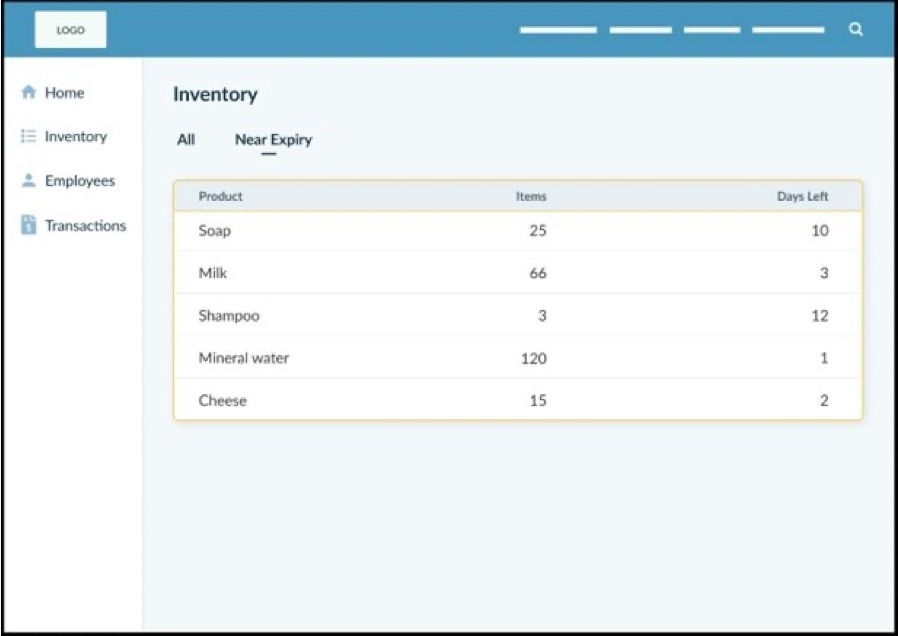
\includegraphics[width=9cm]{Figures/Figma2.jpeg}
  \caption{Inventory tab in the system}
\label{}
\end{figure}

    \item Mobile access for inventory management: A store employee can use the mobile app to access inventory data, update inventory levels, and perform inventory management tasks from anywhere, allowing for more flexibility in managing inventory.

    \begin{figure}[H]
  \centering
   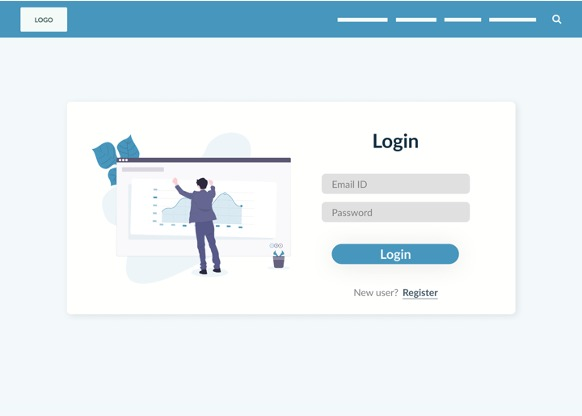
\includegraphics[width=9cm]{Figures/Figma4.jpeg}
  \caption{Login page}
\label{}
\end{figure}

\begin{figure}[H]
  \centering
   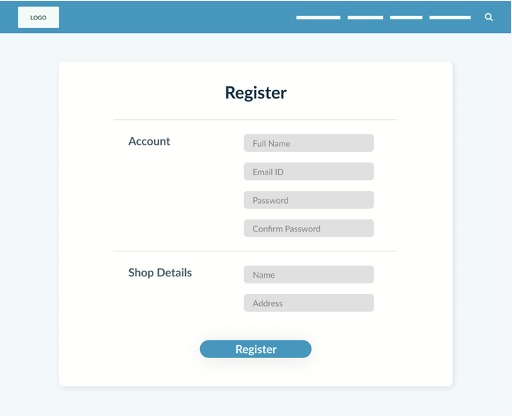
\includegraphics[width=9cm]{Figures/Figma3.jpeg}
  \caption{Registration Page}
\label{}
\end{figure}

\begin{figure}[H]
  \centering
   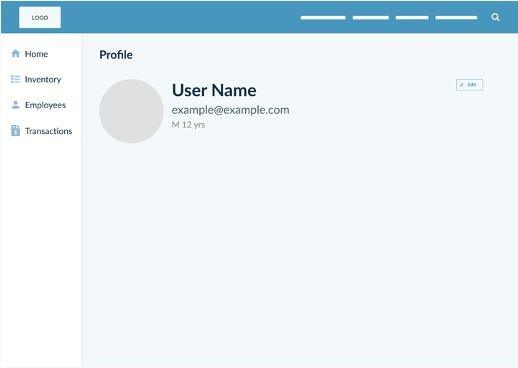
\includegraphics[width=9cm]{Figures/Figma6.jpeg}
  \caption{User profile}
\label{}
\end{figure}

    \item Customizable alerts for inventory issues: A store manager can set up customizable alerts for low inventory levels, stockouts, and other inventory-related issues, receiving notifications via email, SMS, or in-app notifications.

    
    \begin{figure}[H]
  \centering
   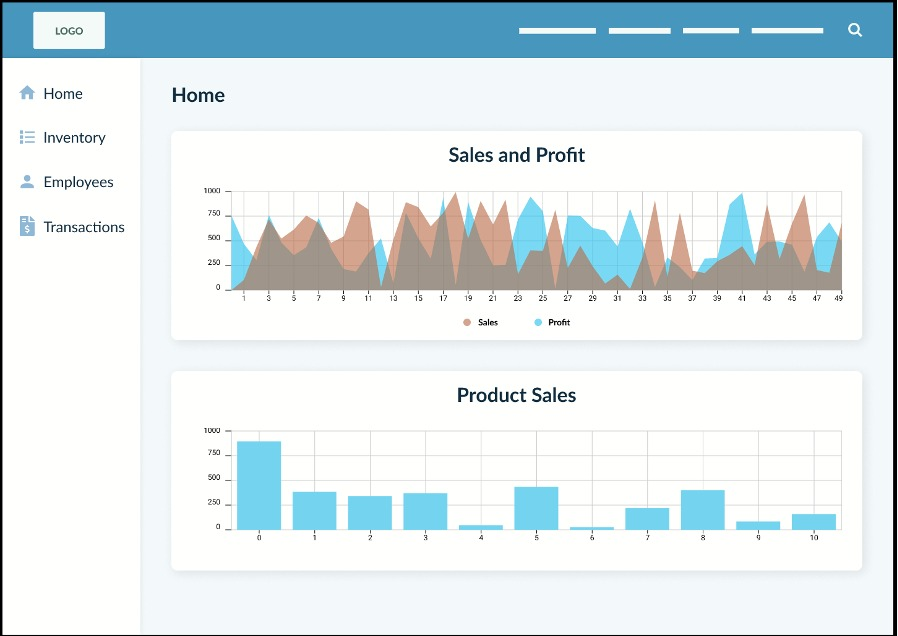
\includegraphics[width=9cm]{Figures/Figma1.jpeg}
  \caption{Homepage of the system}
\label{}
\end{figure}

    \item Automatic updates based on sales transactions: When a customer makes a purchase using the POS system, the inventory management system automatically updates inventory levels, ensuring accurate inventory tracking and reducing errors related to manual data entry.

    \begin{figure}[H]
  \centering
   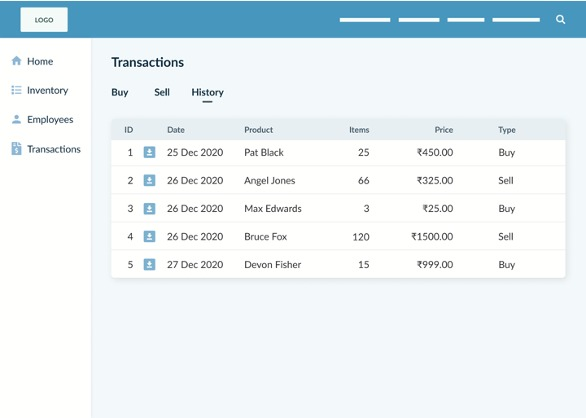
\includegraphics[width=9cm]{Figures/Figma7.jpeg}
  \caption{Transactions History tab}
\label{}
\end{figure}

\begin{figure}[H]
  \centering
   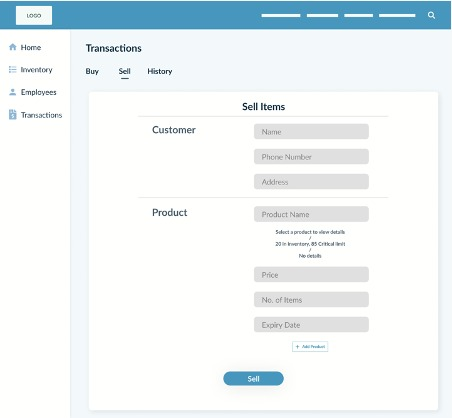
\includegraphics[width=9cm]{Figures/Figma8.jpeg}
  \caption{Transaction Details for selling items}
\label{}
\end{figure}

\begin{figure}[H]
  \centering
   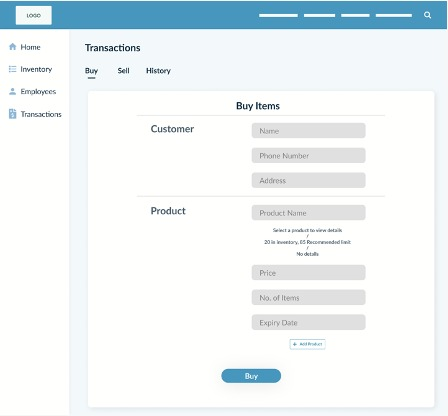
\includegraphics[width=9cm]{Figures/Figma5.jpeg}
  \caption{Transaction Details for buying items}
\label{}
\end{figure}

    \item Managing vendor relationships: A store manager can use the vendor management functionality to track vendor performance, manage purchase orders, and ensure timely delivery of goods, improving the efficiency of the purchasing process and reducing inventory-related issues.
\end{enumerate}
\newpage